% sol.tex - Report for IAML assignment

\documentclass{report}
\usepackage{times}
\usepackage[T1]{fontenc}
\usepackage[margin=2.5cm]{geometry}
\usepackage{graphicx}
\usepackage{cite}
\usepackage{url}
\usepackage[small,labelfont=it,textfont=it]{caption}
\usepackage{subfig}
\usepackage{listings}
\usepackage{longtable}
\begin{document}
\title{Assignment - IAML Fall 2011}
\author{Josh Reese\\s1129936}
\maketitle
\begin{center}{\bf \LARGE{A}}\end{center}
(i)\\
\begin{table}[h]
  \centering
  \begin{tabular}{|c|c|c|c|}
    \hline
    {\bf Classifier} & {\bf NaiveBayes} & {\bf Junction Tree} & {\bf SVM}\\
    \hline
    {\bf \% Correct} & 12 & 37 & 46\\
    \hline
  \end{tabular}
  \citation{Results on {\bf train\_faces.arff}}
  \label{table}
\end{table}\\
(ii)\\
Since we have ten classes (distinct faces) it would seem reasonable to
create ten clusters. Two things of note when examining the clusters are
that the amount of records in the clusters is extremely imbalanced
with the majority of the records being located in two separate
clusters and that different faces are placed in the same cluster.\\
\begin{figure}[h]
  \centering
  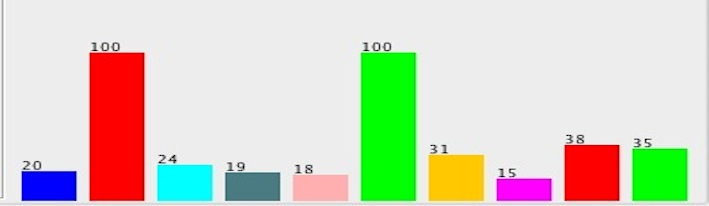
\includegraphics[height=25mm]{images/AiiClusters.jpg}
  \caption{Number of records allocated to each cluster using 10 clusters.}
  \label{fig}
\end{figure}\\
\begin{figure}[h]
  \centering
  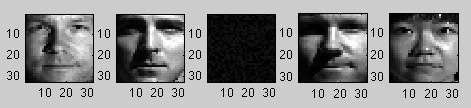
\includegraphics[height=25mm]{images/AiiFaces.jpg}
  \caption{Sample of images from the same cluster.}
  \label{fig}
\end{figure}\\
The classifiers used in part (i) performed so poorly because of the
noise found in the data. We can see from the sample shown in Figure 2
that the data contains blocks of all solid colors as well as faces. If
we take the cluster count to 12 to account for solid black images and
solid white images we can see some more reasonable results. Though the
cluster shown of faces, Figure \ref{fig} in the appendix, is comprised of several different faces at
least there are no solid color in this cluster anymore.\\
(iii)\\
To clean the data I used {\bf RemoveWithValues} on values < 5.0 and >
250.0 and was left with 190
instances. I came up with these numbers by first thinking about what
the problem appeared to be: images which don't contain a face but just
a white or black square. Then, from examining the data in the \emph{Edit}
feature of the \emph{Preprocess} tab, I noticed the images
that had this characteristic of a single color were mostly comprised of
only numbers less than 5.0 or greater than 250.0 (approximately). What
I would really have liked to used would be a filter which filters out
records which have a variance less than some specified variance. With
this tool I could have very effectively filtered out records that were
only black or white.\\
(iv)\\
\begin{center}
  \begin{tabular}{|c|c|c|c|}
    \hline
    {\bf Classifier} & {\bf NaiveBayes} & {\bf Junction Tree} & {\bf SVM}\\
    \hline
    {\bf \% Correct} & 50.5 & 55.8 & 76.3\\
    \hline
  \end{tabular}
\end{center}
A very simple way to compare models is by the percentage of the
training data they have evaluated correctly. Just this small
preprocessing of the data has caused a drastic increase in the
performance of the classifiers. Though it was the Naive Bayes
classifier that had the most noticeable increase. This is, at least in
part, because we
had a number of examples that were duplicated (e.g. all white images),
or redundant, and this is known to have negative effects to the
Naive Bayes learning process~\cite{DM}. See Figure 4.\\
(v)\\
\begin{figure}[h]
  \centering
  \subfloat[Incorrectly classified]{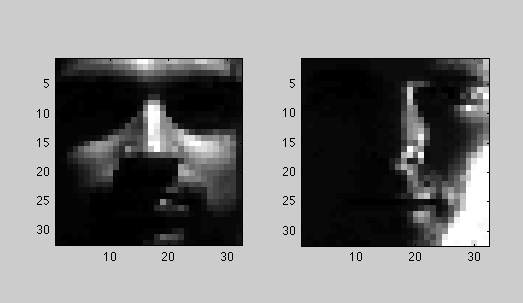
\includegraphics[height=25mm]{images/AvIncorrect.jpg}}
  \subfloat[Correctly classified]{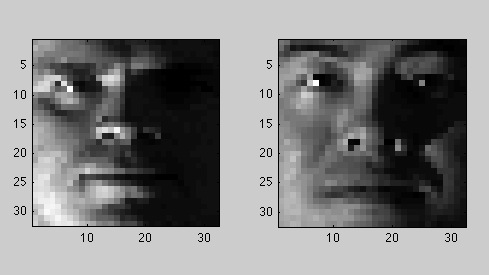
\includegraphics[height=25mm]{images/AvCorrect.jpg}}
  \caption{Results from {\bf SMO} for 1(v)}
  \label{fig}
\end{figure}\\
It would appear that the classifiers have the most trouble when trying
to distinguish faces which contain a lot of black. Though I didn't see
any specific examples I would image this is the same for images with
large amounts of any single color. In the second incorrect example
provided the image is nearly half completely black. This image essentially
only has half the information that a more clear image might have which
is going to make this harder to classify.\\
\begin{center}{\bf \LARGE{B}}\end{center}
(i)\\
The distribution of Naive Bayes, with numeric attributes, is a normal
distribution with the
assumption of independence in the attributes. I do
not really think this is a sensible choice for this data because the
color of pixels in the same region are in fact related and are likely
not distributed normally. If pixel\_1
has the value 0.0 it is very unlikely that pixel\_2 will have the
value 250.0 while it is much more likely to have something close to
0.0.\\
\begin{center}
  \begin{tabular}{|c|c|c|c|c|c|c|c|}
    \hline
    {\bf Number of bins} & {\bf 5} & {\bf 10} &{\bf 20} & {\bf 40} & {\bf 60} & {\bf 80} & {\bf 100}\\
    \hline
    {\bf \% Correct} & 45 & 57 & 61.5 & 62 & 62.5 & 60.5 & 59\\
    \hline
  \end{tabular}
\end{center}
\begin{figure}[h]
  \centering
  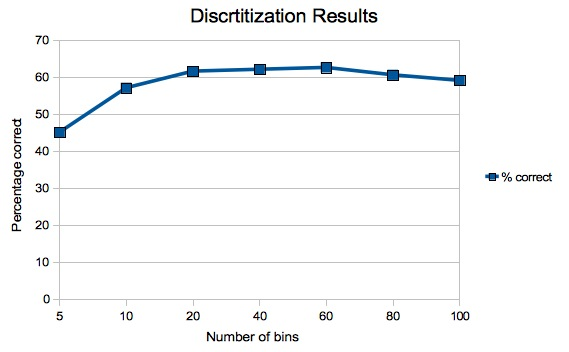
\includegraphics[height=55mm]{images/BiGraph.jpg}
  \caption{Results of using Naive Bayes on bins of different size}
  \label{fig}
\end{figure}
The important things to consider are what range of pixel values are
significant. Too large a range will bin dissimilar values together while
too small a range will bin similar values into different bins. For
this case the best scenario was 60 bins which produced an accuracy
rate of 62.5\%. In part A we had a Naive Bayes correct percentage rate
of 50.5\% while
with the binning we have maxed the correct percentage at 60 bins and
62.5\%. As I mentioned earlier it looks like after 60 bins the range
of values in each bin became too small for Naive Bayes to work as
intelligently with the data. While the range of values in each bin
prior to 60 bins is too large. Additionally what we have done by
discretizing the data is we have removed the assumption that this is a
normal distribution.\\
(ii)\\
'Attribute evaluator' works by computing the information gain of each
attribute and only selecting those with information gain higher than
the specified threshold. Information gain in weka is calculated using the
following equation:\\
\begin{center}
  \( InfoGain(Class,Attribute) = H(Class) - H(Class | Attribute)\)\\
\end{center}
As a note it is clear that $H(Class) = 1$ for {\bf
  train\_faces\_clean.arff} because we have an equal number of each
class which when plugged into our entropy equation will produce the
maximum entropy:
\begin{center}\(
H(S) = \frac{- \sum_{1}^{10} P(\frac{1}{10})log_{2}(\frac{1}{10})}
  {log_{2}(10)} = 1
\)\end{center}
Where the $log_{2}(10)$ represents the number of bits of entropy in
this system and is used as a normalizer. Weka computes
$H(Class|Attribute)$ by first converting the attribute into a discrete
value.\\
(iii)\\
The pixels with the highest information gain appear to be around the
eyes and mouth mostly, with some scatterings throughout the whole
face. For face
recognition these locations seem to make sense as you can certainly
tell a lot about a face by examining where these pixels are concentrated. One
thing we couldn't do with this representation of the data is, for
example, select faces with similar noses, or scars on their
cheeks. This is because we've lost a lot of information about the
different areas of the face.\\
\begin{figure}[h]
  \centering
  \includegraphics[height=40mm]{images/BiiiFace.jpg}
  \caption{Pixels with the highest information gain.}
  \label{fig}
\end{figure}\\
(iv)\\
\begin{center}
  \begin{tabular}{|c|c|c|c|}
    \hline
    {\bf Classifier} & {\bf NaiveBayes} & {\bf Junction Tree} & {\bf SVM}\\
    \hline
    {\bf \% Correct} & 60 & 63.5 & 91\\
    \hline
  \end{tabular}
\end{center}
The performance of each of the classifiers has increased but the
Support Vector Machine has drastically increased (14.7\%). By removing so
many of the attributes, all of which weren't doing anything but
confusing our classifiers, we have made the job of the classifier
easier. Due to the large increase in the SVM model it is my belief that
these attributes we have removed were primarily located near the
decision boundary for each class. Since we have removed them the SVM
will be able to construct support vectors which more accurately
separate the classes.\\
\begin{center}{\bf \LARGE{C}}\end{center}
Using the provided {\bf train\_faces\_clean.arff} file.\\
(i)\\
Most eigenvalues are below 1 and the majority sit very close to 0 (or
at 0). As we discussed in the lectures this is often the
case. See Figure \ref{fig:eigen}.\\
\begin{figure}[h]
  \centering
  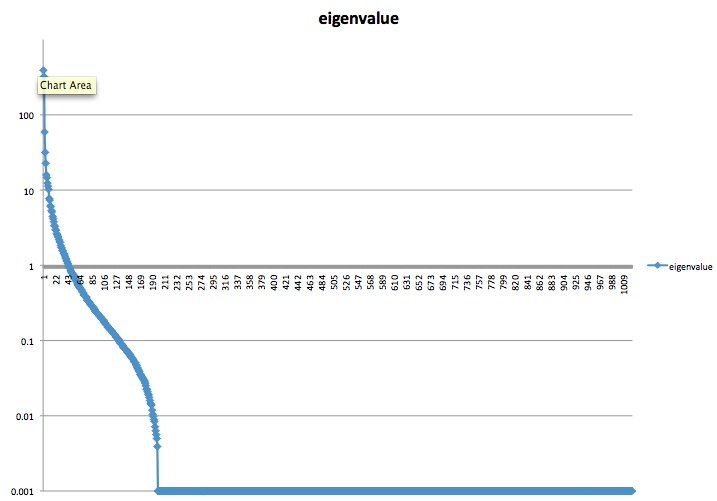
\includegraphics[height=70mm]{images/CiEigen.jpg}
  \caption{Eigenvalues.}
  \label{fig:eigen}
\end{figure}\\
(ii)\\
Processing leaves us with 32 Eigenvectors. Compared to part A the
Naive Bayes and Support Vector Machine classifiers improved significantly
while the Junction Tree classifier improved but much less
drastically. My intuition here is that the Naive Bayes and Support
Vector classifiers benefit from filtering out correlated data (which
is a feature of PCA) while the Junction Tree doesn't benefit quite as
much (which is why Information Gain is generally used in Junction Trees).
\begin{center}
  \begin{tabular}{|c|c|c|c|}
    \hline
    {\bf Classifier} & {\bf NaiveBayes} & {\bf Junction Tree} & {\bf SVM}\\
    \hline
    {\bf \% Correct} & 81.5 & 61.5 & 82.5\\
    \hline
  \end{tabular}
\end{center}
(iii)\\
\begin{figure}[h]
  \centering
  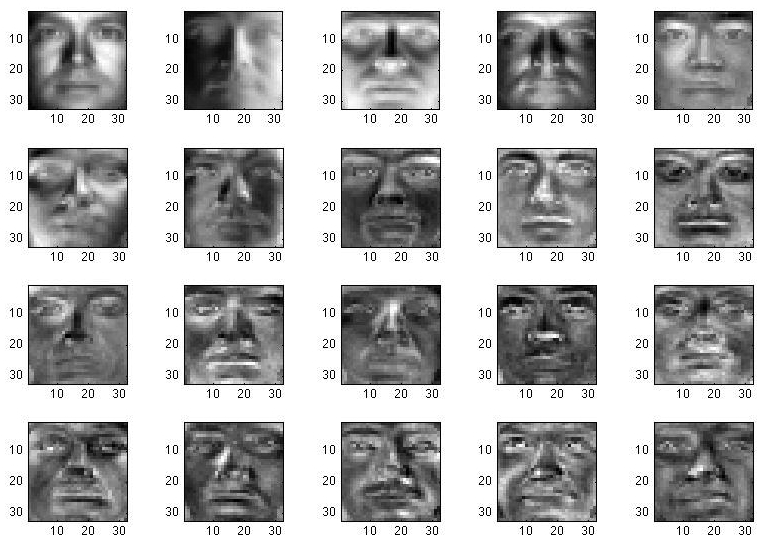
\includegraphics[height=70mm]{images/CiiiFaces.jpg}
  \caption{Top 20 Eigenfaces.}
  \label{fig}
\end{figure}\\
First Eigenvalue: 390.78591\\
Second Eigenvalue: 323.30464\\
The Eigenfaces we have constructed represent the face similarity in
the reduced space. These faces should be insensitive to factors such
as lighting, expression, and orientation and are a weighted
combination of all the faces in the data set. ~\cite{PCA}. If we look
at the first two we notice they are actually the same face with
variations in the lighting. Where the first Eigenface is a pretty
clear picture the second is less clear.\\
(iv)\\
We can reconstruct a recognizable face with 5 components.\\
\begin{figure}[h]
  \centering
  \subfloat[Original face]{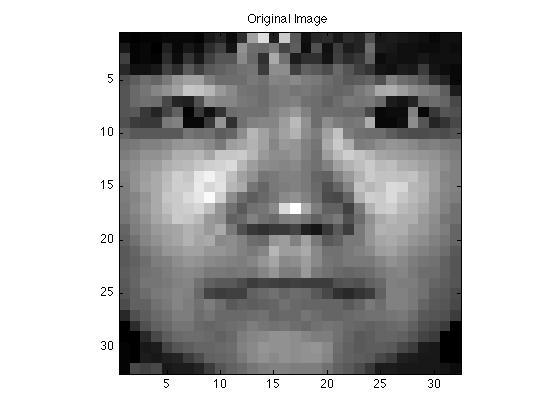
\includegraphics[height=30mm]{images/CivFace0.jpg}}
  \subfloat[Reconstructed face (4 PCs)]{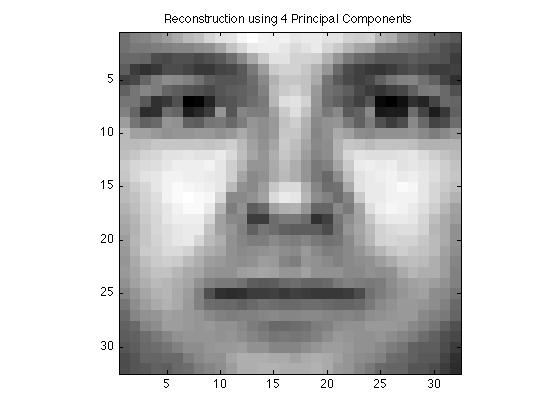
\includegraphics[height=30mm]{images/CivFace2.jpg}}
  \subfloat[Reconstructed face (5 PCs)]{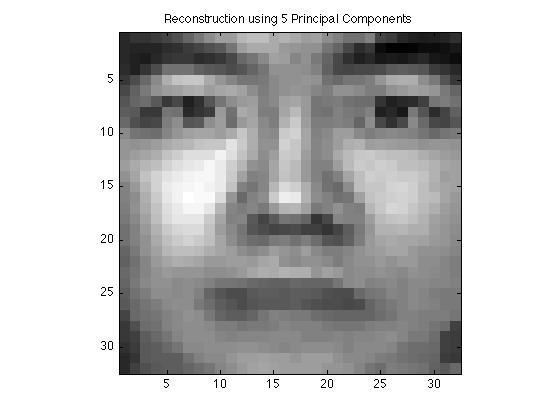
\includegraphics[height=30mm]{images/CivFace1.jpg}}
  \caption{Reconstruction of faces from PCs.}
  \label{fig}
\end{figure}\\
(v)\\
I wouldn't really expect this to matter any more than if we removed
the lowest 4 Eigenvectors. With Naive Bayes we are assuming that all
of the data is independent so all of the Eigenvectors should matter
the same amount. I would expect the classifier accuracy to decrease
just based on the fact we are removing information from our training
examples. However, it would look like the accuracy improves in this
case.\\
\begin{center}
  \begin{tabular}{|c|c|}
    \hline
    {\bf Classifier} & {\bf NaiveBayes}\\
    \hline
    {\bf \% Correct} & 82.5\\
    \hline
  \end{tabular}
\end{center}
(vi)\\
Once we add in components past 40 the percent accurate starts
dropping. We know from earlier that 95\% of the variance is explained
by the first 32 of the Eigenvectors so all we are doing by adding in
these additional Eigenvectors is adding in outliers which are going to
have the effect of causing the support vectors to change thus making
our decision boundary less accurate.\\
\begin{figure}[h]
  \centering
  \includegraphics[height=60mm]{images/Cviplot.jpg}
  \caption{Shows the percentage correctly classified using an SVM.}
  \label{fig}
\end{figure}
\begin{center}{\bf D}\end{center}
(i)\\
\begin{center}
  \begin{tabular}{|c|c|c|c|}
    \hline
    & {\bf NaiveBayes} & {\bf Junction Tree} & {\bf SVM}\\
    \hline
    train\_clean & 53.6(5.95) & 61.90(7.19) & 88.00(3.15)\\
    \hline
    train\_best & 63.6(6.04) & 64.30(7.02) & 90.10(3.19)\\
    \hline
    train\_pca & 79.9(5.80) & 60.10(8.49) & 80.90(4.89)\\
    \hline
  \end{tabular}
\end{center}
When comparing the results using the training sets as the baseline we
get:
\begin{center}
  \begin{tabular}{|c|c|c|c|}
    \hline
    \multicolumn{4}{|c|}{{\bf Confidence: 0.05}}\\
    \hline
    & {\bf train\_clean} & {\bf train\_best} & {\bf train\_pca}\\
    \hline
    Naive Bayes & 53.6(5.95) & 63.60(6.04) V & 79.90(5.80) V\\
    \hline
    Junction Tree & 61.90(7.19) & 64.30(7.02) & 60.10(8.49)\\
    \hline
    SVM & 88.00(3.15) & 90.10(3.19) & 80.90(4.89) *\\
    \hline
  \end{tabular}
\end{center}
\begin{center}
  \begin{tabular}{|c|c|c|c|}
    \multicolumn{4}{|c|}{{\bf Confidence: 0.01}}\\
    \hline
    & {\bf train\_clean} & {\bf train\_best} & {\bf train\_pca}\\
    \hline
    Naive Bayes & 53.6(5.95) & 63.60(6.04) V & 79.90(5.80) V\\
    \hline
    Junction Tree & 61.90(7.19) & 64.30(7.02) & 60.10(8.49)\\
    \hline
    SVM & 88.00(3.15) & 90.10(3.19) & 80.90(4.89)\\
    \hline
  \end{tabular}
\end{center}
From this we can see that the Naive Bayes classifier performs quite
well on the {\bf train\_best} and {\bf train\_pca}. From these results
I would use the train\_best since at 95\% confidence it has 1 win and 2
ties while the {\bf train\_pca} has 1 win, 1 loss, and 1 tie.\\
(ii)\\
Seed: 42\\
\begin{center}
  \begin{tabular}{|c|c|}
    \hline    
    Percent\ Remaining & Percent\ Correct\\
    \hline
    5\% & 21.5\%\\
    \hline
    10\% & 31\%\\
    \hline
    35\% & 79\%\\
    \hline
    50\% & 80.5\%\\
    \hline
    65\% & 91\%\\
    \hline
    80\% & 90\%\\
    \hline
    100\% & 92\%\\
    \hline
  \end{tabular}
\end{center}
\begin{figure}[h]
  \centering
  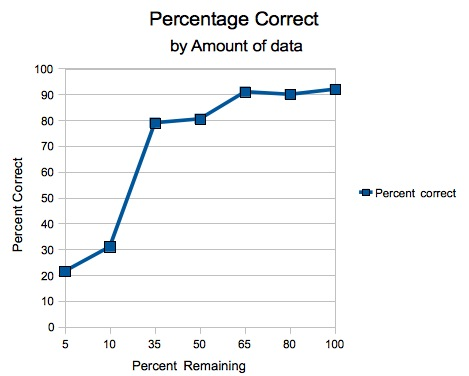
\includegraphics[height=60mm]{images/DiiChart.jpg}
  \caption{Percentage correct by addition of more data.}
  \label{fig}
\end{figure}
It looks at about 65\% of the data the accuracy has plateaued at around 90\%
correct. So, it would appear that adding more data will not really
bring us better performance. If we think about what the SVM is doing
it is looking for an optimal decision boundary between the classes. At
some point the line is going to become relatively constant where
adding more data isn't going to change the decision boundary because
the new data will fall to one side of the boundary. This is known to
have no effect on the classifier because it is only changing the
support vectors that changes how it behaves. We can see
this here at the 65\% to 100\% range where the percentage correct
doesn't really change.\\
(iii)\\
\begin{center}
  \begin{tabular}{|c|c|c|}
    \hline
    {\bf Classifier} & {\bf Naive Bayes \& PCA} & {\bf Naive Bayes \&
      PCA \& Clustering}\\
    \hline
    {\bf \% Correct} & 83.5\% & 85.6\%\\
    \hline
  \end{tabular}
\end{center}
The performance increase from using clustering is 2.1\%. By adding
cluster labels to the PCA representation we have increased the
accuracy of our model, but only slightly.
This student's claim about adding cluster labels is not something with
which I agree. For one we can see this empirically between the results
just obtained (though only in a small degree). Intuitively we can
imagine points when applying PCA and
attempting to classify them with Naive Bayes are still not classified
with a high confidence. Adding a cluster label can give us one more
aspect to take into account for our decision.\\

\begin{center}{\bf E}\end{center}
My first objective for this portion of the assignment was to examine,
very broadly, some techniques that are already in use for facial
recognition and apply those to this set. What I found was that PCA is
a very popular approach to this problem as well as ICA, LDA, EBGM,
SVM, and HMMs (among many others) \cite{PCA0,PCA1,ICA0,LDA0,EBGM,SVM,HMM}. 
Having seen this research and noticing that weka doesn't appear to
support ICA, LDA, EGBM, and HMMs being supported only in a
downloadable module I decided to focus my efforts on trying
different classifiers with PCA and in general see how different
classifiers would respond to the data set.
\begin{table}[h]
  \begin{minipage}[b]{0.5\linewidth}
    \centering
    \begin{tabular}{|c|c|}
      \hline
      \multicolumn{2}{|c|}{{\bf train\_faces\_clean.arff}}\\
      \hline
          {\bf Classifier and settings} & {\bf \% Accurate}\\
          \hline
          SVM with PCA (-R=0.99 -C=3.0) & 93\%\\
          \hline
          SVM (-C=0.2) & 93\%\\
          \hline
          JT48 with clustering (-N=10 -C=0.5) & 71.5\%\\
          \hline
          MultilayerPerceptron & 93.5\%\\
          \hline
          RBFNetwork with PCA (-R=0.99) & 81.5\%\\
          \hline
          Simple Logistic (-P) & 95.5\%\\
          \hline
          Random Forest (-I=1024 -K=100 -depth=50) & 96.5\%\\
          \hline
    \end{tabular}
    \caption{Classifiers trained using {\bf train\_faces\_clean.arff}
      with {\bf val\_faces.arff} as the testing set. Parameters in
      parenthesis represent only the changed parameters.}
    \label{Table 1}
  \end{minipage}
  \hspace{0.6cm}
  \begin{minipage}[b]{0.5\linewidth}
    \centering
    \begin{tabular}{|c|c|}
      \hline
      \multicolumn{2}{|c|}{{\bf train\_faces\_clean\_best.arff}}\\
      \hline
          {\bf Classifier and settings} & {\bf \% Accurate}\\
          \hline
          SVM with PCA (-R=0.99 -C=2.0) & 94\%\\
          \hline
          SVM (-C=0.7) & 94\%\\
          \hline
          JT48 with clustering (-N=10) & 71.5\%\\
          \hline
          RBFNetwork with PCA (-R=0.99 -W=0.9) & 89\%\\
          \hline
          Simple Logistic (-P) & 93.5\%\\
          \hline
          Random Forest (-I=1024 -K=150 -depth=50) & 96.5\%\\
          \hline
    \end{tabular}
    \caption{Classifiers trained using {\bf
        train\_faces\_clean\_best.arff} with {\bf
        val\_faces\_best.arff} as the testing set. Parameters in
      parenthesis represent only the changed parameters.}
    \label{fig}
  \end{minipage}
\end{table}\\
Having come up with the most accurate classifiers I could construct I
then took the two different classifiers with the highest accuracy
(Simple Logistic and Random Forest with {\bf
  train\_faces\_clean.arff}) and combined the training set and
validation set into one file and ran 5 fold cross-validation on the
new set. The results of this test are in \ref{Table 3}. Following this
I ran each of these two classifiers (using the combined {\bf
  train\_faces\_clean.arff} and {\bf val\_faces.arff}) on
{\bf test\_faces.arff} and
compared the difference in predicted values from each
classifier. Given the choice between the two I am more confident in
the Simple Logistic classifier because all of it's error values are
drastically less than those of the Random Forest as shown in Table
\ref{Table 3}. With the two predicted results I ran a python script to
examine each prediction and for each prediction that differed between
the two classifiers output the prediction from the classifier that had
the highest confidence in its prediction as well as which classifier
the new prediction came from. Both the script used for comparison and
a final table of the results generated can be found in the
appendix. As specified the results have also been submitted in the
file iam\_assignment.res (this is the Simple Logistic run).
\begin{table}[h]
  \centering
  \begin{tabular}{|c|c|c|c|c|}
    \hline
        {\bf Classifier} & {\bf \% Accurate} & {\bf RMS Error} &
        {\bf Relative Absolute Error} & {\bf Root Relative Squared
          Error}\\
        \hline
        {\bf Random Forest} & 98.5\% & 0.126 & 35.56\% & 42\%\\
        \hline
        {\bf Simple Logistic} & 98\% & .06 & 2.57\% & 19.59\%\\
        \hline
  \end{tabular}
  \caption{Computed from using 5 fold cross-validation on {\bf
      train\_faces\_clean.arff} joined with {\bf val\_faces.arff}.}
  \label{Table 3}
\end{table}
\newpage
\appendix
\begin{center}{\bf \LARGE{APPENDIX}}\end{center}
\section{Python program}
\lstinputlisting{compare.py}
\section{Results from final testing}
\begin{center}
\begin{longtable}{|l|l|l|l|l|}
  \citation{Results for testing on {\bf test\_faces.arff}}
  \label{Table 4}\\
  \hline
      \multicolumn{1}{|c|}{{\bf Label}}&
      \multicolumn{1}{|c|}{{\bf Simple Logistic}}&
      \multicolumn{1}{|c|}{{\bf Random Forest}}&
      \multicolumn{1}{|c|}{{\bf Combined}}&
      \multicolumn{1}{|c|}{{\bf Winning Classifier}}\\ \hline
      \endfirsthead
      
      \multicolumn{5}{c}%
                  {{\bfseries \tablename\ \thetable{} -- continued from previous page}}\\
                  \hline
  \multicolumn{1}{|c|}{{\bf Label}} &
  \multicolumn{1}{|c|}{{\bf Simple Logistic}}&
    \multicolumn{1}{|c|}{{\bf Random Forest}}&
      \multicolumn{1}{|c|}{{\bf Combined}}&
      \multicolumn{1}{|c|}{{\bf Winning Classifier}}\\ \hline
      \endhead
      \hline
      \multicolumn{5}{|r|}{{Continued on next page}}\\ \hline
      \endfoot
      \hline
      \endlastfoot
1&6:6&6:6&6:6&\\
2&8:8&8:8&8:8&\\
3&9:9&9:9&9:9&\\
4&4:4&4:4&4:4&\\
5&9:9&9:9&9:9&\\
6&7:7&7:7&7:7&\\
7&3:3&3:3&3:3&\\
8&2:2&2:2&2:2&\\
9&9:9&9:9&9:9&\\
10&1:1&1:1&1:1&\\
11&8:8&8:8&8:8&\\
12&6:6&6:6&6:6&\\
13&3:3&3:3&3:3&\\
14&1:1&1:1&1:1&\\
15&8:8&8:8&8:8&\\
16&5:5&5:5&5:5&\\
17&4:4&4:4&4:4&\\
18&6:6&6:6&6:6&\\
19&8:8&8:8&8:8&\\
20&3:3&3:3&3:3&\\
21&3:3&3:3&3:3&\\
22&7:7&7:7&7:7&\\
23&3:3&3:3&3:3&\\
24&2:2&2:2&2:2&\\
25&4:4&4:4&4:4&\\
26&4:4&4:4&4:4&\\
27&5:5&5:5&5:5&\\
28&2:2&2:2&2:2&\\
29&10:10&10:10&10:10&\\
30&3:3&3:3&3:3&\\
31&10:10&10:10&10:10&\\
32&5:5&5:5&5:5&\\
33&7:7&7:7&7:7&\\
34&1:1&1:1&1:1&\\
35&10:10&10:10&10:10&\\
36&8:8&8:8&8:8&\\
37&7:7&7:7&7:7&\\
38&10:10&7:7&10:10&LOG\\
39&3:3&3:3&3:3&\\
40&7:7&4:4&7:7&LOG\\
41&7:7&4:4&7:7&LOG\\
42&6:6&6:6&6:6&\\
43&2:2&2:2&2:2&\\
44&5:5&5:5&5:5&\\
45&7:7&7:7&7:7&\\
46&9:9&9:9&9:9&\\
47&4:4&4:4&4:4&\\
48&4:4&4:4&4:4&\\
49&6:6&6:6&6:6&\\
50&9:9&9:9&9:9&\\
51&5:5&5:5&5:5&\\
52&1:1&1:1&1:1&\\
53&4:4&4:4&4:4&\\
54&8:8&8:8&8:8&\\
55&10:10&10:10&10:10&\\
56&3:3&7:7&7:7&FOR\\
57&9:9&9:9&9:9&\\
58&10:10&10:10&10:10&\\
59&9:9&9:9&9:9&\\
60&8:8&8:8&8:8&\\
61&5:5&5:5&5:5&\\
62&8:8&8:8&8:8&\\
63&1:1&1:1&1:1&\\
64&8:8&8:8&8:8&\\
65&10:10&10:10&10:10&\\
66&8:8&8:8&8:8&\\
67&9:9&7:7&9:9&LOG\\
68&8:8&6:6&8:8&LOG\\
69&7:7&7:7&7:7&\\
70&4:4&4:4&4:4&\\
71&5:5&5:5&5:5&\\
72&7:7&7:7&7:7&\\
73&6:6&6:6&6:6&\\
74&5:5&5:5&5:5&\\
75&1:1&1:1&1:1&\\
76&8:8&8:8&8:8&\\
77&4:4&4:4&4:4&\\
78&3:3&3:3&3:3&\\
79&9:9&9:9&9:9&\\
80&2:2&2:2&2:2&\\
81&1:1&1:1&1:1&\\
82&7:7&7:7&7:7&\\
83&10:10&10:10&10:10&\\
84&5:5&8:8&5:5&LOG\\
85&2:2&2:2&2:2&\\
86&4:4&4:4&4:4&\\
87&2:2&2:2&2:2&\\
88&10:10&10:10&10:10&\\
89&10:10&10:10&10:10&\\
90&6:6&6:6&6:6&\\
91&5:5&5:5&5:5&\\
92&6:6&6:6&6:6&\\
93&4:4&7:7&4:4&LOG\\
94&7:7&7:7&7:7&\\
95&8:8&8:8&8:8&\\
96&2:2&2:2&2:2&\\
97&9:9&9:9&9:9&\\
98&10:10&10:10&10:10&\\
99&6:6&6:6&6:6&\\
100&5:5&5:5&5:5&\\
101&10:10&10:10&10:10&\\
102&7:7&7:7&7:7&\\
103&10:10&10:10&10:10&\\
104&5:5&5:5&5:5&\\
105&8:8&8:8&8:8&\\
106&9:9&9:9&9:9&\\
107&5:5&5:5&5:5&\\
108&8:8&8:8&8:8&\\
109&6:6&6:6&6:6&\\
110&9:9&9:9&9:9&\\
111&1:1&1:1&1:1&\\
112&9:9&9:9&9:9&\\
113&7:7&7:7&7:7&\\
114&6:6&6:6&6:6&\\
115&5:5&5:5&5:5&\\
116&5:5&5:5&5:5&\\
117&4:4&4:4&4:4&\\
118&1:1&1:1&1:1&\\
119&1:1&1:1&1:1&\\
120&2:2&2:2&2:2&\\
121&7:7&7:7&7:7&\\
122&2:2&2:2&2:2&\\
123&3:3&3:3&3:3&\\
124&2:2&2:2&2:2&\\
125&9:9&9:9&9:9&\\
126&5:5&5:5&5:5&\\
127&4:4&4:4&4:4&\\
128&3:3&3:3&3:3&\\
129&1:1&1:1&1:1&\\
130&3:3&10:10&3:3&LOG\\
131&10:10&10:10&10:10&\\
132&1:1&1:1&1:1&\\
133&3:3&3:3&3:3&\\
134&2:2&2:2&2:2&\\
135&3:3&3:3&3:3&\\
136&5:5&5:5&5:5&\\
137&8:8&8:8&8:8&\\
138&6:6&6:6&6:6&\\
139&6:6&6:6&6:6&\\
140&1:1&1:1&1:1&\\
141&4:4&4:4&4:4&\\
142&4:4&4:4&4:4&\\
143&6:6&6:6&6:6&\\
144&6:6&6:6&6:6&\\
145&1:1&1:1&1:1&\\
146&2:2&2:2&2:2&\\
147&3:3&3:3&3:3&\\
148&7:7&7:7&7:7&\\
149&2:2&2:2&2:2&\\
150&1:1&1:1&1:1&\\
151&8:8&8:8&8:8&\\
152&5:5&5:5&5:5&\\
153&9:9&9:9&9:9&\\
154&7:7&7:7&7:7&\\
155&5:5&5:5&5:5&\\
156&3:3&3:3&3:3&\\
157&3:3&7:7&3:3&LOG\\
158&1:1&1:1&1:1&\\
159&10:10&10:10&10:10&\\
160&2:2&2:2&2:2&\\
161&9:9&9:9&9:9&\\
162&8:8&8:8&8:8&\\
163&10:10&10:10&10:10&\\
164&2:2&2:2&2:2&\\
165&2:2&2:2&2:2&\\
166&8:8&8:8&8:8&\\
167&4:4&4:4&4:4&\\
168&10:10&10:10&10:10&\\
169&3:3&3:3&3:3&\\
170&1:1&1:1&1:1&\\
171&3:3&3:3&3:3&\\
172&6:6&6:6&6:6&\\
173&1:1&1:1&1:1&\\
174&2:2&2:2&2:2&\\
175&6:6&6:6&6:6&\\
176&10:10&10:10&10:10&\\
177&3:3&3:3&3:3&\\
178&9:9&9:9&9:9&\\
179&7:7&7:7&7:7&\\
180&2:2&2:2&2:2&\\
181&7:7&7:7&7:7&\\
182&4:4&4:4&4:4&\\
183&1:1&1:1&1:1&\\
184&6:6&6:6&6:6&\\
185&8:8&8:8&8:8&\\
186&10:10&10:10&10:10&\\
187&6:6&6:6&6:6&\\
188&5:5&5:5&5:5&\\
189&4:4&4:4&4:4&\\
190&9:9&9:9&9:9&\\
191&8:8&8:8&8:8&\\
192&9:9&9:9&9:9&\\
193&8:8&8:8&8:8&\\
194&9:9&9:9&9:9&\\
195&10:10&10:10&10:10&\\
196&3:3&3:3&3:3&\\
197&1:1&1:1&1:1&\\
198&5:5&5:5&5:5&\\
199&2:2&2:2&2:2&\\
200&3:3&3:3&3:3&\\
\end{longtable}
\end{center}
\begin{figure}[h]
  \centering
  \subfloat[Distribution of 12 clusters]{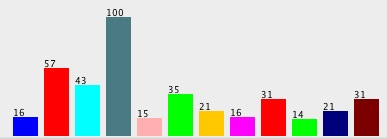
\includegraphics[height=25mm]{images/AiiCluster1_1.jpg}}\\
  \subfloat[Sample from cluster 4]{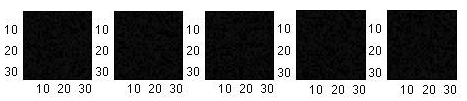
\includegraphics[height=25mm]{images/AiiCluster0.jpg}}\\
  \subfloat[Sample from cluster 2]{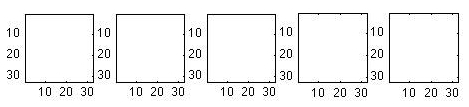
\includegraphics[height=25mm]{images/AiiCluster1.jpg}}\\
  \subfloat[Sample from cluster 1]{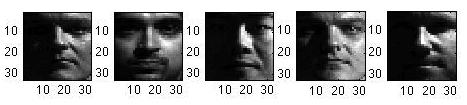
\includegraphics[height=25mm]{images/AiiFaces1.jpg}}\\
  \caption{Results from A(ii) using 12 clusters.}
  \label{fig}
\end{figure}
\bibliography{sol}{}
\bibliographystyle{plain}
\end{document}
